\documentclass{beamer}
%%%%%%
% Self-contained copy of the decision theory slides that were originally part of
% the Agent Foundations presentation
% (agent foundations/projects/Agency_presentation/main.tex). They were moved out
% of that deck and saved here as reference material for the future Decision
% Theory presentation. The preamble below is a minimal, logo-free reproduction
% of the Agency deck's block style so that this file compiles on its own.
%%%%%%

\usepackage[utf8]{inputenc}
\usepackage[english]{babel}
\usepackage{amsmath,amssymb}

\definecolor{gris}{rgb}{0.92,0.92,0.92}
\definecolor{blau-upc}{rgb}{.192,.365,.506}
\setbeamercolor{titlelike}{fg=blau-upc}
\setbeamertemplate{itemize items}[circle]
\setbeamercolor{item}{fg=blau-upc}
\setbeamertemplate{blocks}[rounded][shadow=true]
\setbeamercolor*{block body}{bg=gris}
\setbeamerfont{block body}{size=\footnotesize}
\setbeamercolor*{block title}{parent=structure,bg=blau-upc,fg=white}
\setbeamertemplate{navigation symbols}{}

\title{Decision Theory \\ {\large (slides extracted from the Agent Foundations deck)}}
\author{Daniel C}
\date{}

\begin{document}

\frame{\titlepage}

\frame{\frametitle{Embedded Subproblem: Decision Theory}
	\begin{block}{The problem of counterfactuals for embedded agents}
		{\tiny
		\begin{itemize}
			\item For a dualistic agent (playing a video game), optimization is simple: just $\arg\max_a \mathbb{E}[U \mid \text{do}(A=a)]$ over actions
			\item For embedded agents, which action you pick is just another fact about the world. There is no well-defined notion of ``what would happen if I took a different action''
			\item Different decision theories correspond to different ways of constructing these counterfactuals: conditioning on the action as evidence (EDT), intervening causally on it (CDT), or reasoning about the logical consequences of being the kind of agent that runs a given decision procedure (FDT).
		\end{itemize}
		}
	\end{block}

}
\frame{\frametitle{Causal decision theory}
	\begin{block}{Causal decision theory and the do-calculus}
		{\tiny
		\begin{itemize}
			\item A Bayesian network encodes conditional independences via a directed acyclic graph. The joint distribution factorizes as:
			$$P(X_1, \ldots, X_n) = \prod_{i=1}^{n} P(X_i \mid \text{Pa}(X_i))$$
			where $\text{Pa}(X_i)$ are the parents of $X_i$ in the graph
		\end{itemize}
		\begin{center}
			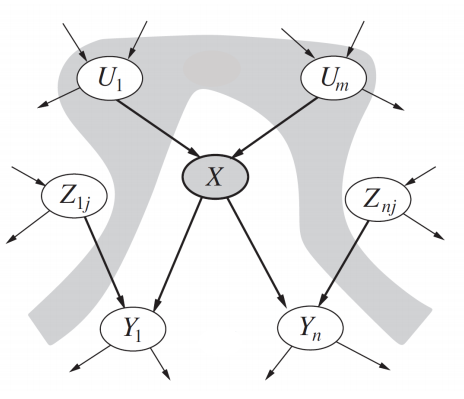
\includegraphics[width=0.17\linewidth]{bayesnet.png}
		\end{center}
		\begin{itemize}
			\item The $\text{do}$-operator models an intervention: $\text{do}(X = x)$ \textit{severs} all incoming arrows to $X$ (removing the influence of $X$'s parents) and fixes $X = x$, then propagates consequences downstream:
			$$P(Y \mid \text{do}(X = x)) = \sum_{u, z} P(Y \mid X{=}x, U{=}u, Z{=}z)\, P(U{=}u)\, P(Z{=}z)$$
			\item CDT chooses $a^* = \arg\max_a \mathbb{E}[U \mid \text{do}(A = a)]$: intervene on the action node and maximize expected utility under the resulting distribution
		\end{itemize}
		}
	\end{block}

}

\frame{\frametitle{Functional Decision Theory}
	\begin{block}{Twin Prisoner's Dilemma}
		{\tiny
		\begin{itemize}
			\item You and your psychological twin must each choose to cooperate or defect. You reason identically but choose in separate rooms without communication
			\item \textbf{CDT reasoning:} ``My action cannot causally affect my twin's action. No matter what she does, I gain extra by defecting. Defection dominates cooperation.'' Both defect.
			\item But your twin is computing the \textit{same decision function}. If your decision procedure outputs ``defect'', so does hers. The relevant question is not ``what should I do holding her action fixed?'' but ``what output of this decision procedure would yield the best outcome?''
		\end{itemize}
		}
	\end{block}
	\begin{block}{FDT: reasoning about the logical output of your decision procedure}
		{\tiny
		\begin{itemize}
			\item FDT asks: ``Which output of this very decision function I'm using would yield the best outcome, given everything in the world that depends on this function's output?''
			\item In the twin PD: if this function outputs cooperate, both copies would cooperate. If it outputs defect, both would defect. So FDT cooperates
			\item  FDT is sensitive to whether the correlation between your action and the world arises from a \textit{logical dependence}. It acts as if it controls both its own action and the action of its copy.
			\item FDT performs well in environments that contain copies of you, or predictors that model your decision procedure -- precisely the settings that arise for embedded agents
		\end{itemize}
		}
	\end{block}
}

\frame{\frametitle{Updateless Decision Theory}
	\begin{block}{Reflective stability of decision theories}
		{\tiny
		\begin{itemize}
			\item We want decision theories to be \textit{reflectively stable}: the decision theory shouldn't want to self-modify into a different decision theory
			\item CDT defects in the twin prisoner's dilemma, but \textit{before entering the game}, a CDT agent would pay to precommit to cooperating -- it would like to self-modify into an FDT agent. This means CDT is not reflectively stable
		\end{itemize}
		}
	\end{block}
	\begin{block}{From updateful to updateless}
		{\tiny
		\begin{itemize}
			\item \textbf{Updateful (EDT):} choose the action that maximizes expected utility \textit{given your current observations}:
			$$\texttt{choice}(o) := \arg\max_{a \in A}\; \mathbb{E}_P[U \mid \texttt{choice}(o) = a,\; O = o]$$
			\item \textbf{Updateless (UDT):} drop the conditioning on observations -- choose the action you would have wanted to commit to \textit{before} seeing anything:
			$$\texttt{choice}(o) := \arg\max_{a \in A}\; \mathbb{E}_P[U \mid \texttt{choice}(o) = a]$$
		\end{itemize}
		}
	\end{block}

}
\frame{\frametitle{Updateless Decision Theory}
\begin{block}{UDT as coordination across counterfactual branches}
		{\tiny
		\begin{itemize}
			\item \textbf{Blackmail:} giving in to blackmail achieves higher utility \textit{when you're being blackmailed}. But giving in incentivizes blackmail -- so an updateful agent conditions gives in to blackmail when it is being blackmailed.
			\item UDT asks: ``what \textit{policy} (mapping from observations to actions) would I have wanted to commit to before seeing any observations?'' Being the kind of agent that refuses blackmail is the better policy overall, even though it is locally costly when blackmailed
			\item  UDT agent coordinates across all counterfactual branches: by refusing to give in, the blackmailed branch sacrifices utility so that the branches where blackmail is never attempted becomes more probable. The overall policy maximizes expected utility across all branches, evaluated from the prior
			\item UDT is reflectively stable: a UDT agent would not want to self-modify into something else, because it is already following the policy it would have chosen to commit to from the start
		\end{itemize}
		}
	\end{block}
    }

\end{document}
